\chapter{Implementation}
\label{chapter:implementation}

This chapter will describe the implementation of the tool.
In particular, I will outline the high-level architecture of
the software, discuss the internal representation of
LCL problems as well as the representation of the query object.
Moreover, I will discuss how the batch classification has been
implemented. Finally, at the end of the chapter, I will cover
several miscellaneous items such as the problem normalization
algorithm, integration of the Round Eliminator tool into
my software, and some of the properties of the Web interface,
which has also been implemented as a part of the thesis project.

\section{The high-level architecture of the tool}

This section will outline the high-level architecture of the tool and
will describe in further detail some of its most important
components. Despite the chapter's name, I am not going
to describe low-level implementation detail in this section,
but instead, try to convey a technical perspective on the tool
as a whole. I will also discuss and critically analyze some
of the architectural and technological decisions that have been
made during the implementation phase.

On the high level, the software consists of three parts:
front-end application, back-end application, and a database.
The database contains arguably the most important component
of this project: the definitions of LCL problems as well as their
known upper and lower bounds. The back-end part contains
the core logic for classifying LCL problems. Besides, it acts
as a middle layer between the database and the front-end part.
That is, it is responsible for receiving data from one of the
components (e.g.\ database), transforming it to the
format understandable by the other part (e.g.\ the front end),
and finally sending it to that part. Finally, the
front-end part's main responsibility is to provide
an understandable and user-friendly user interface
through which one could classify individual LCL problems
as well as query for the whole families of problems
that satisfy specified criteria. Furthermore,
the client-side part of the application is
responsible for displaying the results returned by the
back-end part in a concise and understandable manner.
For the depiction of the high-level architecture of the
implementation, refer to Figure~\ref{fig:implementation-architecture}.

\begin{figure}[ht]
  \begin{center}
    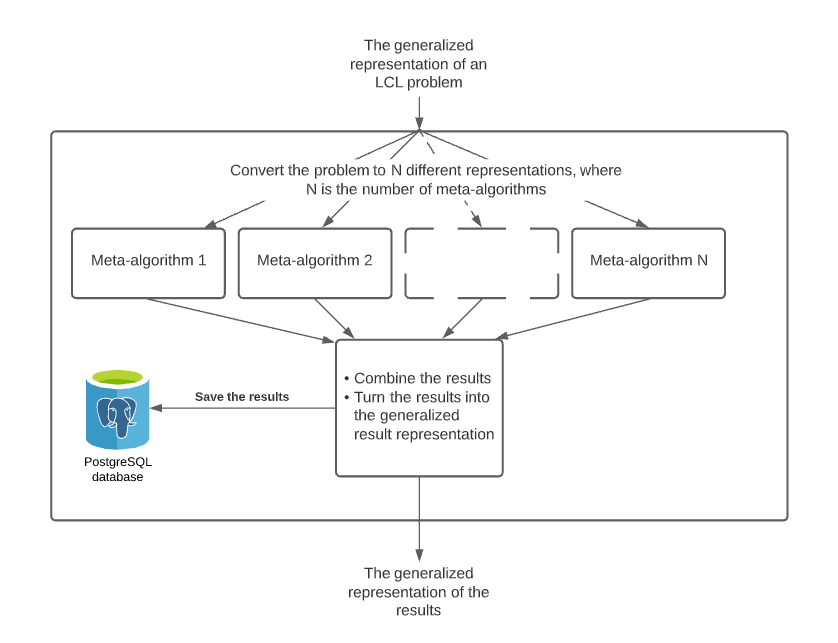
\includegraphics[width=\textwidth]{images/tool-architecture.png}
    \caption{The high-level architecture of the implementation}
    \label{fig:implementation-architecture}
  \end{center}
\end{figure}

The database contains only three tables: one for
storing LCL problems together with their upper and
lower bounds, one for keeping track of what families of
problems have been generated and classified via batch
classification mechanisms, and one storing meta-data
of the meta-algorithms used in classifying the LCLs.
The front end is quite simple from a technical perspective
too. Some of the details about the client-side of the
application will be discussed more in Section~\ref{section:webinterface}.
The back end, however, contains most of the complexity of
the tool. Therefore, in this section, I will concentrate
mainly on the server-side.

\subsection{Problem}

The core element of the whole application and the
back-end part, in particular, is the Problem class.
For representing an LCL problem, I have decided
to use a notation similar to that of Round
Eliminator. My representation, however, also
allows for graph types other than trees -- namely cycles.
Besides, it allows the underlying graph of a problem
to be rooted (or directed in the case of cycles).
Finally, it allows representing problems where
leaves' and root's output labels are also constrained.
The representation similar to that of a Round
Eliminator has been chosen because of its generality.
In particular, as I have shown in Theorem~\ref{theorem:re_formalism_is_general},
any LCL problem
on $(\beta, \delta)$-biregular unrooted trees -- provided
that nodes of degrees other than $\beta$ and $\delta$ are unconstrained
and nodes near leaves are unconstrained -- can be represented
using the formalism used in the Round Eliminator.

Since we are only concerned with problems on regular trees and cycles
this representation works well for us. For the cases of cycles,
the only restriction is that degree of both passive and
active configurations has to be two. Also, the case
of directed (rooted) cycles (trees) can be handled
using the \emph{colon notation} that has been already
previously used in a recent paper on automating
the classification of LCLs in rooted trees~\cite{Balliu2021}.
Furthermore, the cases when \emph{irregular} nodes, i.e.\ leaf
nodes or root node, are restricted can also
be handled by specifying those restrictions
(separately for leaf nodes and a root node)
as separate properties of the Problem object.
Thus, my representation of LCL problems is general
enough to cover all the LCL problems that are
included in the scope of the project.

Having explained this, I can finally list all the
properties that are encapsulated into the
Problem object. The object contains the already
mentioned active configuration, passive configurations,
leaf constraints (which can be an empty set), root constraints
(which can be an empty set too), as well as special flag variables
indicating whether all active or all passive configurations
are allowed for active and passive nodes respectively.
If one of the two flag variables is set to true,
it overrides whatever is contained in the variables
holding the actual active and passive configs.
Besides, each problem object contains information
on the type of the underlying graph: path, cycle, or
tree. Notice that although any path is always a tree,
I chose to differentiate between those two
for convenience. It is worth mentioning that
a path graph type will be chosen as an internal
representation whenever both active and
passive configurations are of degree two and
the user-selected graph type is not cycle.
In particular, if a user specifies a tree as a graph
type and provides configurations of degree two,
a tree will still be chosen as a graph type of the problem
internally. Finally, after parsing the configs
that are always provided in a string format,
the tool automatically decides whether the given problem's
underlying graph is rooted/directed or not.

It is also worth noting that as the first step of
creating a Problem object, the specified parameters,
including nodes' configurations and constraints
are checked for validity. Thus, if, for example,
a problem is misspecified so that some of the
configurations are ``directed'' while others are not,
an exception is thrown containing a message with
a human-readable explanation for why the
specification was invalid. After the validity
of the specification is checked, a problem is
normalized by executing the normalization algorithm
described below in Section~\ref{section:problem-normalization}.

\subsection{Classification}

Another central component of the back end is
a function responsible for classifying LCL problems.
On the high level, the function takes as input an LCL problem and
runs underlying meta-algorithms, some of which might be
able to provide some useful information about the complexity of the
problem. After that, the function combines the results
returned by all the meta-algorithms. Based on the results returned,
the function determines the tightest known lower and upper bounds of
the LCL problem both in the deterministic and randomized LOCAL
models. Finally, a Response object is constructed based on the bounds
and is returned as the function's result. In the best case, tight
complexity bounds are found for both deterministic and randomized
settings. In the worst case, trivial bounds are returned:
\emph{unsolvable} for upper bounds and $\Omega(1)$ for lower bounds.

Each of the underlying meta-algorithms or datasets is wrapped
in a function -- I will refer to it as \emph{subclassify} from now on -- such
that it provides a unified interface for the main
\emph{classify} function. In particular, subclassify takes
as input an instance of the Problem class and
returns an instance of the Response class. A Response object
simply encapsulates upper and lower bounds for both
deterministic and randomized settings. There is
exactly one subclassify function for each meta-algorithm
or dataset that I use. Inside each subclassify function,
I first check if the provided problem can be classified
at all by the underlying meta-algorithm. Often, we can
exit early already at this stage if, for example, the meta-algorithm
in question deals only with rooted trees and the provided input is a 
problem on unrooted trees (or e.g.\ a problem on cycles). Then,
if we have not exited the function yet,
we transform an instance of the Problem class to a problem
representation used by the meta-algorithm that the given
subclassify function wraps around. The meta-algorithm is then executed,
the returned result is transformed into an instance of the
Response class and the Response object is returned as
a result of the subclassify function. Once the subclassify
function is called for each of the meta-algorithms,
the results of the calls are combined, and
a single Response object is returned from the
classify function.

\subsection{Query}

The query class encapsulates some of the properties
based on which the database is queried for problems.
Only problems that satisfy the provided Query object will be
returned. The properties encapsulated by a Query object are
more or less directly mapped to an SQL query's WHERE clause.
The Query class groups those properties into three parent items:

\begin{itemize}
  \item problem properties,
  \item complexity bounds,
  \item include/exclude configuration.
\end{itemize}

\emph{Problem properties} define a family of problems that are to be
returned from the database. It includes the following fields:

\begin{itemize}
  \item active degree,
  \item passive degree,
  \item alphabet size (an upper bound on it to be precise),
  \item whether active/passive configurations are necessarily monochromatic
  (meaning that only such configurations are allowed where the same label is outputted
  on all ports by a single node, e.g. $\{A,~A,~A\}$, or $\{B,~B,~B,~B\}$, etc.
  Note that different nodes can still output different labels on their ports,
  as long as the labels are the same on the ports of a single node. For example,
  some node $v$ can output $A$
  on all its ports, while some node $u$ can output $B$ on all its ports.),
  \item whether the underlying graph is directed/rooted or not,
  \item the type of the underlying graph, which is always one of the following three
  options: tree, cycle, path.
\end{itemize}

\emph{Complexity bounds} limit the returned problems further by
restricting their complexities. The \emph{complexity bounds} object
contains the following items:

\begin{itemize}
  \item an upper bound in the randomized LOCAL setting (referred to as RUB),
  \item a lower bound in the randomized LOCAL setting (referred to as RLB),
  \item an upper bound in the deterministic LOCAL setting (referred to as DUB),
  \item a lower bound in the deterministic LOCAL setting (referred to as DLB).
\end{itemize}

The restriction of the fetched problems is done according to the
following logic: only those problems are returned (not filtered out)
whose known randomized upper bound is at most as high as RUB, whose
known randomized lower bound is at least as high as RLB, whose
known deterministic upper bound is at most as high as DUB and whose
known deterministic lower bounds is at least as high as DLB. Notice that
for a problem not to be filtered out, all four criteria must be
satisfied.

Finally, \emph{include/exclude configuration} has the following
items encapsulated in it:

\begin{itemize}
  \item Whether only the smallest problem has to be returned (in terms of the number of configurations).
  \item Whether only the largest problem has to be returned (in terms of the number of configurations).
  \item Whether only those problems must be returned whose randomized upper
  and lower bounds do not match.
  \item Whether only those problems must be returned whose deterministic upper
  and lower bounds do not match.
  \item Whether only those problems must be returned whose randomized both
  upper and lower bounds are trivial (i.e.\ unsolvable and $\Omega(1)$
  respectively).
  \item Whether only those problems must be returned whose deterministic both
  upper and lower bounds are trivial (i.e.\ unsolvable and $\Omega(1)$
  respectively).
  \item List of configurations $L$ such that if a problem's configurations contain at least one configuration from $L$, the problem is excluded. Note that
  the item has no effect if left empty.
  \item List of configurations $L$ such that if a problem's configurations contain all of the configurations from $L$, the problem is excluded. Note that
  the item has no effect if left empty.
  \item List of configurations $L$ such that if a problem's configurations contain at least one configuration from $L$, the problem is included.
  Otherwise, a problem is excluded.
  Note that
  the item has no effect if left empty.
  \item List of configurations $L$ such that if a problem's configurations contain all of the configurations from $L$, the problem is included.
  Otherwise, a problem is excluded.
  Note that
  the item has no effect if left empty.
\end{itemize}

\section{Problem normalization}
\label{section:problem-normalization}

This section describes the above-mentioned problem normalization
algorithm. The algorithm is used for determining which problems
are equivalent to each other. This, in turn, allows us
to reduce the amount of needed storage. Besides, this prevents
situations when a tool needs to run classification for a problem $A$
from the very beginning while an isomorphic problem $B$ has already been classified
by the tool previously and saved in the database. Thus, the normalization
algorithm also allows us to reduce the usage of computational resources.

The algorithm is based on the problem normalization algorithm
from the Round Eliminator~\cite{Olivetti2020}. While the original
algorithm is written in Rust programming language, I
reimplemented it in Python and changed some of its
implementation details to better suit my purpose.
However, the general idea of the algorithm stays the same.

The reason why I chose the normalization algorithm in my solution
to be heavily based on the algorithm from the Round Eliminator~\cite{Olivetti2020}
is primarily due to
the fact that the Round Eliminator's problem representation is very similar to the problem
representation used in my solution. Furthermore, the normalization
algorithm used in the Round Eliminator is known to be correct and works
sufficiently fast for the Round Eliminator to be useful for the research community.
While it is perhaps true that better, more efficient normalization
algorithms exist, I decided to avoid optimizing prematurely and,
as the first iteration, selected a working, "good enough" algorithm.
If and when the current implementation of normalization will start
causing performance problems, it should be relatively easy to
switch to another more efficient normalization algorithm.

First, we determine how many labels are used in the description of the
problem $P$ i.e.\ its alphabet size. Then, we map each letter in the description
to a letter from A to Z. For example, if integers were used for describing
the problem, the integers will be mapped to capital letters of
the English alphabet. It is important to point out already now that
one limitation of the current implementation is the fact that
a problem with more than 26 labels cannot be normalized correctly.
Once we obtain the list of letters used, we calculate all
the permutations of the list. For each permutation, we execute the following
subroutine:

\begin{enumerate}
  \item Based on the given permutation, create a mapping from each
  element of the problem's alphabet to each symbol in the permutation.
  That is, we map the $i$'th letter of the $P$'s alphabet to the $i$'th symbol
  in the permutation for all $i$ from 1 to the size of $P$'s alphabet.
  \item Based on the obtained mapping, do the following with the problem's
  active configurations, passive configurations, leaf constraints, and
  root constraints one at a time.
  
  \begin{enumerate}
    \item For each line of the configurations/constraints, rename the symbols
    according to the mapping constructed above.
    \item If the problem $P$ is specified on an unrooted/undirected graph,
    change the positions of all symbols on each line of the configurations/constraints according to the symbols' alphabetical order.
    If the underlying graph of $P$ is directed/rooted, keep the currently first
    symbol as the first (this is because it is assumed that the first configuration symbol in configurations of LCLs on directed/rooted graphs always points towards a predecessor/parent node, so its position must be preserved), but change the positions of all the other symbols (again separately for each line)
    according to the symbols' alphabetical order.
    \item If at this point, some configuration lines are
    duplicated, remove all the duplicates so that each configuration
    line is unique.
    \item Sort the unique configuration lines in alphabetical order
    treating the lines as strings.
  \end{enumerate}

  \item Return the newly constructed active configurations,
  passive configurations, leaf constraints, and root constraints as
  a tuple of four elements.
\end{enumerate}

Each execution of the subroutine described above yields a tuple
of size four. Thus, after executing the subroutine on each permutation of
the labels, we eventually obtain a list of tuples of size four.
Then we sort the list and take its first element. The four
elements of this first tuple are then assigned to the $P$'s
active configurations, passive configurations, leaf
constraints, and root constraints, respectively.

% \begin{algorithm}
% \DontPrintSemicolon
% \caption{\label{alg:normalize}normalize($P$)}
% \KwIn{problem $P$}
% \KwOut{problem $P$ with its constraints and configurations normalized}

% $lc \gets$ number of labels in $P$ \;
% $ls \gets$ first $lc$ capital letters of English alphabet \;
% $perms \gets$ a list of all permutations of $ls$  \;
% $all_normalized \gets$ empty array \;
% \For{every $perm$ in $perms$} {
%     add $normalizeForPermutation()$ $all_normalized \;
% }

% this is just an example 


% \Repeat{$R_{i} = R_{i-1}$}{
%   $i \gets i + 1$\;
%   $R_{i} \gets R_{i-1}$\;
  
  
% \uIf{$(\Sigma_\Pi,a \neq \epsilon) \in R_i$ and $\Pi$ is non-empty}{
%   \Return $\Sigma$
%   }
% \Else{
%   \Return $\epsilon$
% }
% \end{algorithm}


\section{Batch classification and reclassification}

This section describes how the batch classification and
batch reclassification mechanisms have been implemented.
Batch classification is important since we want the database
to be pre-populated with a significant number of classified
problems already before the first users start using it.
In particular, we would need to classify huge but finite
families of problems consisting of tens and hundreds of
thousands of LCL problems. Moreover, once a family of
problems is selected, the problems of the family need to
be generated and turned into instances of Problem class before
we can classify them. Batch reclassify functionality,
on the other hand, is needed for cases when, for one reason
or another, we would want to reclassify a certain
family of LCL problems that is already stored in the
database. For example, if I integrate a new meta-algorithm
into my solution in the future, I would need to reclassify
all problem families that are compatible with the newly integrated
meta-algorithm. Or perhaps, a programming mistake has been
made when integrating one of the meta-algorithms, and therefore,
the problems need to be reclassified again.

One option for implementing batch reclassification
mechanisms would be to simply delete all of the problems
of the class in question from the database and execute
the batch classification logic from the beginning
including its first step of generating the problems
of the problem class. However, this is suboptimal,
since the generation of problems of a certain family
usually takes significantly longer times than
the subsequent classification step. For this reason,
I decided to have separate functionality for
batch reclassification.

The batch classification process starts with creating
an object that specifies a family of problems to be
generated, classified, and stored in the database.
The specification includes properties like
active and passive degrees, label count, type of the
underlying graph, etc. The problems of the given
family are then generated via the following algorithm:

\begin{enumerate}
  \item Based on the specified label count, get a list of
  all symbols i.e.\ the alphabet of the problem family.
  \item Based on the alphabet and the specified active/passive
  degrees, generate lists of all the possible
  active and passive one-line configurations.
  \item Get a list of all possible combinations
  of active one-line configurations and a list of all possible
  combinations of passive one-line configurations. The combinations
  can be of any size. This can be accomplished via
  the \emph{powerset} function. Now we have lists of
  all possible active and passive configurations.
  \item Remove empty configurations.
  \item Generate all possible tuples of size two
  where the first element is an active configuration and
  the second is a passive configuration. This corresponds
  to the Cartesian product between the previously generated
  lists of all active and passive configurations.
  \item Remove tuples that have exact duplicates in the
  generated list of tuples, so that all tuples are unique.
  \item Turn each tuple into a Problem object using
  elements of the tuple as active and passive configurations.
  \item Normalize all the problems.
  \item Now that all the problems are in a normalized 
  representation, it is easy to detect whether any two
  problems are isomorphic to each other. Remove such
  problems from the list so that the list contains
  unique non-isomorphic problems only.
  \item Return the list of the newly-generated problems.
\end{enumerate}

Once the problems are generated, they are inserted into the database,
even though they are not classified yet. This is done mainly
because the database will automatically associate a unique
identifier with each of the problems.

After that, the problems are classified. Notice that
some of the meta-algorithms provide a way to classify
lists of problems at the same time, which is often
significantly faster than classifying one problem at a time.
This is due to the fact that some meta-algorithms
(e.g.\ TLP classifier and BRT classifier) are
huge datasets of pre-classified problems. When
classifying each problem individually, such
meta-algorithms would need to read out the whole
dataset from the disk, find one specific problem,
and return the result. On the other hand, when
classifying multiple problems at the same time,
numerous optimizations can be applied e.g.\ reading the 
dataset from the disk just once and search for all
the requested problems at the same time. For this reason,
when batch classifying families of problems, the program first
calls such batch classification methods of meta-algorithm
if such methods exist. Once this is done, a modification
of the previously-described classify function is called
for each individual Problem object. The difference is
that if a meta-algorithm $A$'s batch classify method has been
already called, its subclassify function is not called
anymore during the individual-problem classification which
can significantly speed up the whole batch classification
functionality. Finally, when all problems have been classified,
the database is updated with the classification results.

The batch reclassification functionality resembles
what has been described above with the exception that,
once a family of problems has been specified, it is
not generated but is instead queries from the database.
After that, the fetched problems undergo the same
batch classification process. Finally, the database is
updated with the received classifications.

\section{Integration of the Round Eliminator}

This section describes how the Round Eliminator
tool~\cite{Olivetti2020} has been integrated into my solution.
Before the integration, I had considered several options:

\begin{itemize}
  \item Using an API of a server that runs the back end of the Round Eliminator tool.
  \item Calling the Round Eliminator as a command-line tool from my Python
  application and then parsing the output, which is returned
  in a text format via stdout~\cite{stdio}.
  \item Compiling the Round Eliminator's source code to a ``Shared Object'' file (.so extension)
  using CPython ~\cite{CPython} bindings and then importing the compiled
  functions to my Python application as CPython dependency.
\end{itemize}

At the moment of writing the thesis, the Round Eliminator tool
is deployed using WASM~\cite{WASM}. This virtually means that
there is no back-end part running on a server, but instead,
all of the logic is executed on the client-side of the application.
Redeploying the tool with a standalone server and a separate client
part did not seem like a feasible alternative since this would
require a nontrivial amount of work from the tool's maintainers.
Thus, the first option was not feasible.

On the other hand, the second option was feasible. Indeed,
this method of using the Round Eliminator had already been used in the
implementation of TLP Classifier~\cite{Rocher2020clas}. However,
this approach has several crucial disadvantages.
Firstly, the overhead of calling a command-line command
from a Python program is significant compared to just calling
a Python function. Secondly, the output of the Round Eliminator
would have to be parsed from the plain text format, which
would have added additional complexity to the software.
Finally, the approach complicates the distribution and
deployment process of
the software. Indeed, one would have to install the specific
version of Rust programming language as well as download and
build from source codes the specific version of the Round Eliminator required.

Instead, I have decided to go with the latter option. This
alternative does not have any of the disadvantages listed
in the previous paragraph while being just as feasible and
easy to implement. Compiled in this manner, the whole of the
Round Eliminator logic is contained in a single .so file
that can be easily deployed to e.g.\ a production server.
Besides, the speed improvement is significant: I was
able to execute up to three rounds of the Round Eliminator
in under 100 milliseconds. Finally, the functions
exposed via the .so file, return python-native
data structures so that no additional parsing is required on my side.
This, in turn, has been achieved by adding CPython bindings
to the Round Eliminator source code. The bindings wrap the relevant functions
written in Rust, thus enabling us to pass Python data structures
as parameters and receive the return values as python-interpretable values.
The bindings were implemented using the rust-cpython library~\cite{RustCPython}.


\section{Web interface}
\label{section:webinterface}

This section will briefly discuss some implementation details of
the client-side of the application. First, I start by explaining why
the web interface has been implemented in the first place and why it
is important. Then, I describe some of the technologies that were
chosen as part of the implementation. Finally, I describe the
reasoning behind and advantages of the forms' state being stored
as a query part of the URL.

The reason why I decided to spend additional time and implement
the web interface can be best understood when considering
another tool that has recently been rising in popularity among
the distributed algorithms community -- the Round Eliminator~\cite{Olivetti2020}. The tool has proved to be a very useful utility
when doing research connected to LCL problems on biregular trees.
However, if it was not for the web interface that Olivetti has
implemented, it is most likely that the popularity and
frequency of use of the tool would have been nowhere near the current
levels. Indeed, almost all users of the tool use it via the web
client. Otherwise, a user would need to install Rust programming
language~\cite{Rust}, build the tool locally using the tool
called Cargo~\cite{Cargo} and then run it using a command line.
It is clear that the number of people willing to do that would be
significantly smaller than the number of people who ended up using
an easy-to-use web interface that requires no installation or 
configuration.

By analogy, we can assume with high confidence that significantly more
users would be willing to use my tool via the web interface rather
than downloading the source of the tool locally and installing
a specific version of Python programming language~\cite{CPython}.
Moreover, the richness of the web user interface allows us to convey complicated
ideas related to distributed computing in a way that is easier to understand, at least for a knowledgeable audience. Thus, it is has been
decided to spend some time resources -- even though they were 
quite limited -- on implementing a web user interface that is
relatively easy to use and understand compared to its
command-line-based analog.

The web interface consists of two forms. One form for classifying
individual problems, and another one for issuing queries
about groups of problems against the database. When using the
first form, the application will first check if the requested
problem can be found in a database. If not, it will proceed to
run the classifiers (which corresponds with the classify function described above) and will eventually return the newly
classified result. If the classification result is not trivial (which means that lower bounds are constant and upper bounds are unsolvable),
it will also be stored in the database. The second form, once
submitted, will be transformed into the previously described
\emph{Query} object. The query will then be executed against the database,
the results will be returned to the client-side and rendered
in a user-friendly format.

As a programming language for the front-end application, I decided
to use TypeScript~\cite{TypeScript}, which is a general-purpose
programming language developed and maintained by Microsoft. It
is closely related to JavaScript programming language, which
has become the de facto standard programming language for the Web.
As a framework for the client application, I decided to use
Svelte~\cite{Svelte}. Svelte is an open-source front-end framework
written in TypeScript. Among other things, it allows a simplified
approach for application state management and reduces initial
page load times compared to other front-end frameworks~\cite{SvelteVsReactBundleSize}.

For the styling of the front end, I used a minimalist CSS framework
called Milligram~\cite{Milligram}. It provides a good starting point
when it comes to styling a modern web application. Besides, the total
size of the framework is just 2 kilobytes when zipped~\cite{Milligram}.
This, simplicity to use, and my previous positive experience with
the framework were the decisive factors that influenced my final
choice.

As a final interesting piece of technology used, I describe properties
and the reason for choosing to use svelte-virtual-list~\cite{svelte-virtual-list}.
The library allows rendering only a part of the content instead of rendering
the whole of the content on a web page. In the given case, this is
particularly useful as it allows us to
show tens of thousands of LCL problems (returned as part of the described above querying functionality) in a virtual list.
The virtual list, implemented via the above-mentioned svelte-virtual-list library, renders only a small number (about 3--4)
LCL problems at the same time. At the same time, it allows users to
scroll through the list of problems with no noticeable delay.
If not for the library, the client application would have to render
tens of thousands of LCL problems all at once. This would result in
the user interface freezing for a prolonged period of time (up to several minutes).

Finally, I will explain the reasoning behind and benefits of
storing the state of the two forms as part of the URL's query
component. When searching for interesting query results, or even
just classifying different individual LCL problems, it is often
required to demonstrate the results to somebody else. To allow for such
sharing, I decided to encode the state of both forms in the URL.
Thus, once e.g.\ the results of a query are obtained, it is possible
to copy the link and simply send it to, for example, a colleague.
When opening the link, both forms will be prefilled with
exactly the same values as those of the sender. This will make sure
that, in most cases, the sender and the receiver of the link will end
up with the same results displayed. Besides, if a particularly
interesting query has been discovered, it is possible to
simply copy and store the link. Opening the link in the future,
will prefill the forms with the same parameters and display
the same relevant results.
